\begin{frame}
    \frametitle{State}
        \begin{itemize}
        \item HTTP, the protocol for transferring data between the server and the client, is stateless
        \item Example: HTTP doesn't manage information about pages previously visited by the client, i.e., any URL can be requested by the client at any time. 
        \item If statefulness is required (e.g., page B shall only be served if the client has previously visited page A), the web application must manage a \textit{session}
    \end{itemize}
\end{frame}

\begin{frame}
    \frametitle{statefulness: Web Shop Example}
    \begin{itemize}
        \item Malicious user adds items into the shopping cart
        \item She then skips the page where credit card information must be entered and proceeds directly to the checkout page
        \item If the web application doesn't enforce the correct sequence of pages, the user would successfully place an order without having entered any payment details 
    \end{itemize}
\end{frame}

\begin{frame}
    \frametitle{Managing State Information}
    There are two options to manage state information in web:
    \begin{itemize}
        \item the state information is stored on the server; the users are identified using a \textit{session ID}
        \item the state information is stored on the client
    \end{itemize}
\end{frame}

\begin{frame}[fragile]
    \frametitle{Hidden Input Fields}
    State information can be located in hidden input fields, e.g., 
    \begin{center}
        \begin{verbatim}
            <input name="id" value="1234" type="hidden">        
        \end{verbatim}
    \end{center}

    Such data fields can be easily manipulated using a tool like ZAP-Proxy or using web developer tools in the web browser. Thus, an attacker can easily manipulate hidden input fields. 
\end{frame}

\begin{frame}
    \frametitle{Hidden Input Fields: Finding Vulnerabilities}
    For every hidden input field in the application, you must examine whether the web application's behavior changes if the values of these input fields are altered.

    A classical anti-pattern (luckily not so common anymore) is the use of hidden input fields for storing item price in a web shop. Yet another example is the storage of the user's status, e.g., a signed in user instead of a "guest" or administrator instead of a standard user.
\end{frame}

\begin{frame}
    \frametitle{Hidden Input Fields: Protecting Against Attacks}
    \begin{itemize}
        \item Core issue with hidden input fields: state information is stored \textit{on the client} where it can be easily manipulated by a malicious user
        \item Main defense philosophy: \textit{never trust the client}
        \item Critical information must always be stored on the server
        \item Values received from the client must always be checked \& validated
        \item If values must be stored on the client (e.g., session IDs), they should be encrypted or hashed
    \end{itemize}     
\end{frame}

\begin{frame}
    \frametitle{URL Parameters}
    \begin{itemize}
        \item (State) information can be transmitted in the URL
        \item In contrast to forms, transmitting information via URL parameters does not require clicking a submit button
    \end{itemize}
\end{frame}

\begin{frame}[fragile]
    \frametitle{URL Parameters: Finding Vulnerabilities}
    \begin{itemize}
        \item Using URL parameters to transmit information is a threat, because it is trivial to manipulate them
        \item Look for URL parameters identified during the recon phase
        \item Investigate what happens when you change these parameters. Does this cause an unexpected and unintended change of the state of the web application?
        \item \verb|http://www.webapp.example/editprofile.php?id=123|
        \item What happens when you change \verb|id|? Can you edit the profile of a different user?
        \item Are there (hidden) parameters to activate debug information, e.g., \verb|debug=on|, \verb|debug=1| or \verb|debug=true|?
    \end{itemize}
\end{frame}

\begin{frame}
    \frametitle{URL Parameters: Defending Against Attacks}
    \begin{itemize}
        \item Core issue with URL parameters: state information is stored \textit{on the client} where it can be easily manipulated by a malicious user
        \item URL parameters must always be checked \& validated
        \item If possible, they should be encrypted or hashed
    \end{itemize}
\end{frame}

\begin{frame}
    \frametitle{Cookie Parameters}
    \begin{itemize}
        \item For a long time, cookies were the only option to persistently store data on the client
        \item It is still the prevailing solution
        \item Cookies are frequently used for user identification, e.g., at consecutive visits of a web application
        \item Attacks based on cookie manipulation are called \textit{cookie poisoning}  
    \end{itemize}
\end{frame}

\begin{frame}[fragile]
    \frametitle{Cookies}
    \begin{itemize}
        \item Persistent vs non-persistent cookies
        \item \verb|secure| vs \verb|HttpOnly| cookies
        \item Persistent cookies are stored on client's hard drive as long as their date is validated
        \item Non-persistent cookies are stored in RAM and are deleted when the web browser is closed
        \item \verb|secure| cookies are transmitted only via an HTTPS connection
        \item \verb|HttpOnly| cookies are transmitted via HTTP or HTTPS, but cannot be accessed by JavaScript
    \end{itemize}
\end{frame}

\begin{frame}
    \frametitle{Cookie Parameters: Storage and Manipulation}
    \begin{itemize}
        \item All web browsers store cookies in known file system locations and in known formats
        \item An attacker can easily manipulate this data before it is used by a web application
        \item It is possible to manipulate cookies \textit{on the fly}, e.g., using a tool like the ZAProxy
    \end{itemize}
\end{frame}

\begin{frame}
    \frametitle{Cookie Parameters: Storage and Manipulation}
    \begin{itemize}
        \item Unlike with URL parameters, the attacker can also manipulate the date when the cookie expires, i.e., she can manipulate the cookie's lifetime
        \item In general, cookies can give you access to things like sessions, profiles, etc.
    \end{itemize}
\end{frame}

\begin{frame}
    \frametitle{Cookie Parameters: Storage and Manipulation}
    Example:
    \begin{itemize}
        \item \texttt{weather.xyz} offers detailed weather information against payment
        \item \texttt{weather.xyz} uses cookies that contain \texttt{userID} to identify users
        \item The cookie is valid for the user's subscription period, e.g., a month
        \item Information stored in the cookie is processed by \texttt{weather.xyz} without additional authentication
        \item Attack 1: malicious user manipulates \texttt{userID} to access \texttt{weather.xyz} as another user
        \item Attack 2: malicious user extends their subscription by manipulating the cookie expiration date (by changing the Unix-timestamp in the cookie)
        \item Attack 3: cookies often store the number of failed login attempts. When they reach a specific threshold, say 5, \texttt{weather.xyz} deactivates that user account for 10 minutes to protect against brute force attacks. The attacker bypasses this defense by setting the value of failed login attempts to 0 after each login attempt. Since this can be easily automated, brute force attacks become trivial.
    \end{itemize}
\end{frame}

\begin{frame}
    \frametitle{Cookie Parameters: Finding Vulnerabilities}
    \begin{itemize}
        \item For every cookie found during recon phase, you must check whether a parameter manipulation results in an illegal state change of the web application
        \item Manipulation should also include cookie parameters like expiration
        \item To detect cookie-related vulnerabilities more efficiently, \textit{decrease} the expiration date and check whether the web application denies its service
        \item As an alternative -- if you have access to the server-side source code of the web application -- check whether the source code uses the cookie expiration date as input parameter
    \end{itemize}
\end{frame}

\begin{frame}
    \frametitle{Cookie Parameters: Defending Against Attacks}
    \begin{itemize}
        \item In general, cookie poisoning -- attacks that manipulate cookies -- cannot be eliminated
        \item Cookies are stored on the client and a malicious user can always manipulate data on the client (even data of other users)
        \item Two prominent attacks in this context are \textit{cross-site-scripting} (XSS) and \textit{cross-site-request-forgery} (CSRF)
        \item Attacker exploits web browser capabilities to set a cookie for a different domain
    \end{itemize}
\end{frame}

\begin{frame}
    \frametitle{Cookie Parameters: Defending Against Attacks}
    \begin{itemize}
        \item As a general rule, never trust data supplied by the client
        \item For example, store subscription's expiration date or the number of failed login attempts on the server
        \item If storing data on the client is unavoidable, encrypt or hash that data
        \begin{itemize}
            \item Question to the audience: why?
        \end{itemize} 
    \end{itemize}
\end{frame}

\begin{frame}
    \frametitle{URL Jumping}
    \begin{itemize}
        \item Eve abuses the intended sequence of web pages. This gives her access to functions that by design must be unavailable at that point in time. 
    \end{itemize}
\end{frame}

\begin{frame}[fragile]
    \frametitle{URL Jumping: An Example}
    In a typical web shop, the intended sequence of transactions -- i.e., pages that a shop's customer visits -- could look something like this:
    \begin{enumerate}
        \item Search for a suitable product at \exurl{catalogue.php}
        \item add an article to the shopping cart at \exurl{add.php}
        \item verify the customer order at \exurl{order.php}
        \item provide shipping information (customer's postal address) at \exurl{shipping.php}
        \item enter credit card information at \exurl{payment.php}
        \item checkout \& finish the order at \exurl{checkout.php}
    \end{enumerate}
\end{frame}

\begin{frame}
    \frametitle{URL Jumping: An Example}
    \begin{itemize}
        \item If \attacker can jump from step 4 (\exurl{shipping.php}) directly to step 6 (\exurl{checkout.php}), she might be able to order an item without paying for it
        \item Another example: \attacker could try to post a message to an online forum with creating an account
        \item In general, \attacker tries to identify URLs that must be called in a specific sequence and tries to manipulate this sequence 
    \end{itemize}
\end{frame}

\begin{frame}
    \frametitle{URL Jumping: Locating the Vulnerabilities}
    \begin{itemize}
        \item Make a complete list of URLs in your web application and whether certain URLs must be called in a specific order
        \item Use information gathered during recon phase
        \item For every URL sequence:
        \begin{itemize}
            \item Call the URLs in the intended order and document the parameters passed to the web application
            \item Diverge from the intended sequence and see what happens. Are there any error messages (e.g., "You first must create a user") or are specific URL/pages not accessible?
            \item If there is no error message and the URLs can be accessed in any order, check whether this represents an actual, exploitable vulnerability
        \end{itemize}
    \end{itemize}
\end{frame}

\begin{frame}
    \frametitle{Defense against URL Jumping}
    \begin{itemize}
        \item URL jumping is a security issue only when the sequence in which URLs are accessed is relevant for the web application
        \item In that case, you need to check that the correct sequence is used, e.g., \texttt{checkout.php} would check if the user previously visited \texttt{payment.php} which, in turn, would check if the user previously visited \texttt{shipping.php}  
    \end{itemize}
\end{frame}

\begin{frame}
    \frametitle{Defending against URL Jumping}
    There are 3 options to identify a previously visited URL:
    \begin{enumerate}
        \item The URL (or the corresponding ID) is stored in a hidden input field or in an URL parameter
        \item The URL (or the corresponding ID) is stored in a cookie
        \item The URL, from which the user is allegedly coming, is compared to the \texttt{Referer} field value in the HTTP header 
    \end{enumerate}
\end{frame}

\begin{frame}[fragile]
    \frametitle{Defending against URL Jumping}
    \begin{itemize}
        \item As shown previously, option 1 (hidden input field) and option 2 (cookie) are insecure as they can be easily manipulate by \attacker
        \item That leaves us with option 3 (\texttt{Referer} value)
    \end{itemize}
    An HTTP request could look like this:
    \begin{center}
        \begin{verbatim}
            Get /checkout.php HTTP/1.1
            Host: www.shop.xyz
            User-Agent: Mozilla/5.0 (Macintosh; U; PPC Mac OS X; de-de) [...]
            Accept: */*
            Accept-Encoding: gzip, deflate
            Accept-Language: de-de
            Connection: keep-alive
            Referer: https://www.shop.xyz/payment.php
        \end{verbatim}
    \end{center}
\end{frame}

\begin{frame}
    \frametitle{Defending against URL Jumping}
    \begin{itemize}
        \item The \texttt{Referer} value is automatically set by the web browser
        \item In case of a bookmark or a direct entry in the web browser's address field the \texttt{Referer} value does not exist in the HTTP header
        \item However, the \texttt{Referer} value can be omitted by the web browser (for privacy reasons), removed from the HTTP request by a proxy or manipulated by \attacker
        \item \texttt{Referer} value can be manipulated using a tool like ZAProxy or using a dedicated client where the individual values of the HTTP header can be defined manually
        \item So \texttt{Referer} value is also insecure
    \end{itemize}
\end{frame}

\begin{frame}
    \frametitle{Defending against URL Jumping}
    \begin{itemize}
        \item In the end, the only effective defense against URL jumping -- similar to other attacks -- is to store state information on the server
        \item Specifically, the information about the visited URLs for each user can be stored temporarily in the web application (or persistently in a database)
    \end{itemize}
\end{frame}


\begin{frame}
    \frametitle{Session Highjacking}
    \begin{itemize}
        \item Numerous attacks can be alleviated by storing state information on the server (instead of client)
        \item In that case, the web application needs a way to identify the user
        \item The notion of a \emph{session} is used to associate state information (stored on the server) to a specific user
        \item The web application assigns each session a unique \emph{session identifier} (session-ID)
    \end{itemize}
\end{frame}

\begin{frame}
    \frametitle{Session Highjacking}
    \begin{itemize}
        \item Session-ID is a number or a combination of numbers and letters that uniquely identifies a session
        \item Session-ID is assigned to the client (user) upon the first HTTP request to the web application
        \item Every subsequent request carries the session-ID so that the web application can identify the client (user) and retrieve the corresponding state information stored on the server
    \end{itemize}
\end{frame}

\begin{frame}
    \frametitle{Session Highjacking}
    \begin{figure}[htb]
        \centering
        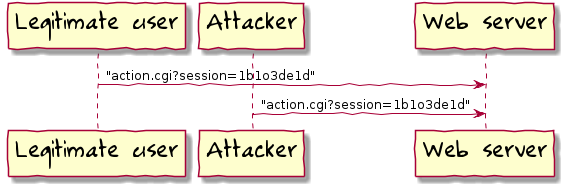
\includegraphics[scale=.5]{uml/session-hijacking.png}
    \end{figure}
    \begin{itemize}
        \item Because the session-ID must be stored on the client, it can be manipulated or stolen
        \item An attack exploiting this vulnerability is referred to as \emph{session hijacking}
        \item \Attacker gets hold of the session-ID information to gain unauthorized access to the web application
    \end{itemize}
\end{frame}

\begin{frame}[fragile]
    \frametitle{Session Highjacking}

    \begin{center}
        \begin{verbatim}
            Name=Alice
            userID=1234
            last=2021-08-24
        \end{verbatim}
    \end{center}

    \begin{itemize}
        \item A special case of session hijacking is the so-called \emph{authorization bypass}
        \item Example: web application identifies the client (user) based on a cookie containing the user name, the user ID and the date of the last session
        \item Is there are user with ID 1235?
        \item \Attacker can change \verb|userID| and use the manipulated cookie to take on the identity of another user
    \end{itemize}
\end{frame}

\begin{frame}
    \frametitle{Finding Session Highjacking Vulnerabilities}
    \begin{itemize}
        \item First, identify the session-ID in the web application, e.g., search for parameters whose names contain \texttt{ID}, \texttt{TOKEN}, \texttt{SESSIONID}, \texttt{ID} or similar strings. These parameters can be located in hidden input fields, URL parameters or in cookies.
        \item Once you identified a potential session-ID, change it and check whether you can impersonate another user
    \end{itemize}
\end{frame}

\begin{frame}
    \frametitle{Defending against Session Highjacking}
    \begin{itemize}
        \item Session hijacking requires a valid session-ID. \Attacker has essentially 4 options to get hold of it:
        \begin{itemize}
            \item Cross-site-scripting (XSS): XSS attacks are commonly used to steal cookies (more on this later). Make sure your web application has no XSS vulnerabilities. In addition, you can set \texttt{HTTPOnly} flag to prevent access to cookies from within JavaScript 
            \item Eavesdropping network traffic: if \attacker can read network traffic between the client and the web application, she can extract the session-ID. Ensure that you web application uses TLS (HTTPS).
            \item Searching logfiles: if \attacker has access to the web server (or proxy) logfiles, she can search them for session-IDs that were transmitted via \texttt{GET} requests. Session-ID should therefore be transmitted in cookies or via \texttt{POST} requests.  
            \item Brute-force attack: \attacker can try to guess the format of your session-IDs and try out various (random) combination until she finds a valid session-ID. You should use large random values as session-IDs.
        \end{itemize}
    \end{itemize}
\end{frame}

\begin{frame}
    \frametitle{Defending against Session Highjacking}
    \begin{itemize}
        \item Performing session identification based on the combination of the session-ID and the IP address of the client makes session hijacking more difficult
        \item Instead of the IP address, you can also use e.g., the \texttt{User-Agent} header (i.e., user the client browser "model" as an additional identification factor)
        \item To reduce session hijacking-related risks, you should end the sessions after a specific time and make the corresponding session-IDs invalid
        \item This can be done using a "hard" time-out (e.g., every session ends after 30 minutes) or a "soft" time-out (e.g., session ends after 10 minutes of inactivity)
    \end{itemize}
\end{frame}


\begin{frame}
    \frametitle{Session Fixation}
    \begin{figure}[htb]
        \centering
        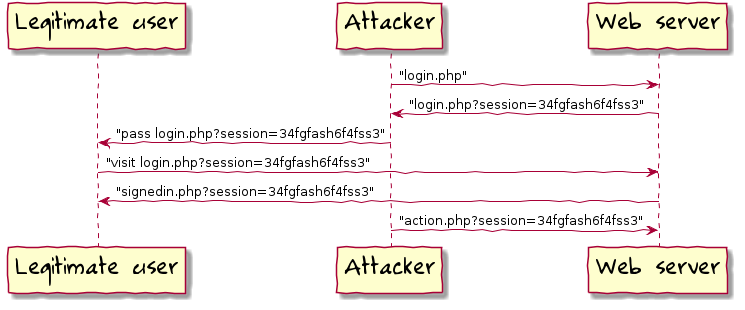
\includegraphics[scale=.5]{uml/session-fixation.png}
    \end{figure}
    \begin{itemize}
        \item Instead of stealing or guessing the session-ID, \attacker attempts to fixate other user's session-ID
        \item Session fixation attacks are typically web based and rely on session identifiers being accepted from URL parameters or POST data
        \item Example: \attacker sends Alice an email with a link to \texttt{login.php?session=34fgfash6f4fss3}
    \end{itemize}
\end{frame}

\begin{frame}
    \frametitle{Finding Session Fixation Vulnerabilities}
    \begin{itemize}
        \item Use the information from the recon phase to identify session-IDs
        \item Call the web application with a session-ID that is already used, i.e., has been set by the web application
        \item Example: if the entry to the web application is \texttt{www.examle.xyz} and the web application, in turn, returns \texttt{www.example.xyz/index.php?session=[valid-session-ID]}, call this URL directly
        \item If you can login and your session-ID is \texttt{[valid-session-ID]}, you've found a session fixation vulnerability
        \item If session-ID is transmitted in a cookie, use ZAProxy to manipulate it   
    \end{itemize}
\end{frame}

\begin{frame}
    \frametitle{Defending against Session Fixation}
    \begin{itemize}
        \item Make sure your web application generates a new, random session-ID each time a user logs in
        \item The same behaviour must be implemented when a new users signs up
        \item Some web applications accept arbitrary session-IDs, i.e., session-IDs that they have not generated
        \item This makes Eve's life easier because she doesn't need to obtain a valid session-ID
        \item Thus, your web application should only accept session-IDs that it actually generated 
        \item Make sure it's impossible to reactivate expired sessions with known "old" session-IDs. If a session expired, a new session must be created with a new session-ID and a new state. Otherwise Eve can mount replay attacks.
        \item You should also leverage the information in HTTP header's \texttt{Referer} field. If the observed sequence of URLs doesn't match the expected sequence, either URL jumping is taking place or two clients (users) are using the same session-ID
    \end{itemize}
\end{frame}